\documentclass[]{article}
\usepackage{lmodern}
\usepackage{amssymb,amsmath}
\usepackage{ifxetex,ifluatex}
\usepackage{fixltx2e} % provides \textsubscript
\ifnum 0\ifxetex 1\fi\ifluatex 1\fi=0 % if pdftex
  \usepackage[T1]{fontenc}
  \usepackage[utf8]{inputenc}
\else % if luatex or xelatex
  \ifxetex
    \usepackage{mathspec}
    \usepackage{xltxtra,xunicode}
  \else
    \usepackage{fontspec}
  \fi
  \defaultfontfeatures{Mapping=tex-text,Scale=MatchLowercase}
  \newcommand{\euro}{€}
\fi
% use upquote if available, for straight quotes in verbatim environments
\IfFileExists{upquote.sty}{\usepackage{upquote}}{}
% use microtype if available
\IfFileExists{microtype.sty}{%
\usepackage{microtype}
\UseMicrotypeSet[protrusion]{basicmath} % disable protrusion for tt fonts
}{}
\usepackage[margin=1in]{geometry}
\usepackage{color}
\usepackage{fancyvrb}
\newcommand{\VerbBar}{|}
\newcommand{\VERB}{\Verb[commandchars=\\\{\}]}
\DefineVerbatimEnvironment{Highlighting}{Verbatim}{commandchars=\\\{\}}
% Add ',fontsize=\small' for more characters per line
\usepackage{framed}
\definecolor{shadecolor}{RGB}{248,248,248}
\newenvironment{Shaded}{\begin{snugshade}}{\end{snugshade}}
\newcommand{\KeywordTok}[1]{\textcolor[rgb]{0.13,0.29,0.53}{\textbf{{#1}}}}
\newcommand{\DataTypeTok}[1]{\textcolor[rgb]{0.13,0.29,0.53}{{#1}}}
\newcommand{\DecValTok}[1]{\textcolor[rgb]{0.00,0.00,0.81}{{#1}}}
\newcommand{\BaseNTok}[1]{\textcolor[rgb]{0.00,0.00,0.81}{{#1}}}
\newcommand{\FloatTok}[1]{\textcolor[rgb]{0.00,0.00,0.81}{{#1}}}
\newcommand{\CharTok}[1]{\textcolor[rgb]{0.31,0.60,0.02}{{#1}}}
\newcommand{\StringTok}[1]{\textcolor[rgb]{0.31,0.60,0.02}{{#1}}}
\newcommand{\CommentTok}[1]{\textcolor[rgb]{0.56,0.35,0.01}{\textit{{#1}}}}
\newcommand{\OtherTok}[1]{\textcolor[rgb]{0.56,0.35,0.01}{{#1}}}
\newcommand{\AlertTok}[1]{\textcolor[rgb]{0.94,0.16,0.16}{{#1}}}
\newcommand{\FunctionTok}[1]{\textcolor[rgb]{0.00,0.00,0.00}{{#1}}}
\newcommand{\RegionMarkerTok}[1]{{#1}}
\newcommand{\ErrorTok}[1]{\textbf{{#1}}}
\newcommand{\NormalTok}[1]{{#1}}
\usepackage{graphicx}
\makeatletter
\def\maxwidth{\ifdim\Gin@nat@width>\linewidth\linewidth\else\Gin@nat@width\fi}
\def\maxheight{\ifdim\Gin@nat@height>\textheight\textheight\else\Gin@nat@height\fi}
\makeatother
% Scale images if necessary, so that they will not overflow the page
% margins by default, and it is still possible to overwrite the defaults
% using explicit options in \includegraphics[width, height, ...]{}
\setkeys{Gin}{width=\maxwidth,height=\maxheight,keepaspectratio}
\ifxetex
  \usepackage[setpagesize=false, % page size defined by xetex
              unicode=false, % unicode breaks when used with xetex
              xetex]{hyperref}
\else
  \usepackage[unicode=true]{hyperref}
\fi
\hypersetup{breaklinks=true,
            bookmarks=true,
            pdfauthor={},
            pdftitle={Statistical Inference : Project},
            colorlinks=true,
            citecolor=blue,
            urlcolor=blue,
            linkcolor=magenta,
            pdfborder={0 0 0}}
\urlstyle{same}  % don't use monospace font for urls
\setlength{\parindent}{0pt}
\setlength{\parskip}{6pt plus 2pt minus 1pt}
\setlength{\emergencystretch}{3em}  % prevent overfull lines
\setcounter{secnumdepth}{0}

%%% Use protect on footnotes to avoid problems with footnotes in titles
\let\rmarkdownfootnote\footnote%
\def\footnote{\protect\rmarkdownfootnote}

%%% Change title format to be more compact
\usepackage{titling}
\setlength{\droptitle}{-2em}
  \title{Statistical Inference : Project}
  \pretitle{\vspace{\droptitle}\centering\huge}
  \posttitle{\par}
  \author{}
  \preauthor{}\postauthor{}
  \predate{\centering\large\emph}
  \postdate{\par}
  \date{20th April 2015}




\begin{document}

\maketitle


\section{Part 2 - Analyse ToothGrowth
Data}\label{part-2---analyse-toothgrowth-data}

This report analyzes the ToothGrowth data in the R datasets package.

Inspection of the data identifies the size of the dataset, names of
variables, type of data and which data fields are categorical.

Inpsection of the data tells us\\1. 60 observations are recorded.\\ +
``len'' (Length of tooth growth)\\ + ``sup'' (Type of supplement used)\\
+ ``dose'' (size of dosage)\\2. there are two types of supplement
used.\\ + ``OJ'' = Orange Juice\\ + ``VC'' = Ascorbic Acid\\3. There are
three dosage levels used. (0.5, 1, 2)

Plot 1 shows three levels of dosage, statistical analysis is needed to
show how dosage is related to growth rate and the confidence levels of
any proposed conclusions.

Plot 2 (refer Appendix) shows us the following.\\* at low (0.5mg) and
medium (1mg) doses more tooth growth is observed with Orange Juice than
with ascorbic acid.\\* at high (2mg) doses the variance in tooth grown
observed is higher with ascorbic acid than with Orange Juice.\\* In both
cases higher doses indicate higher tooth growth.\\* outliers exist for
the Orange Juice @ 2mg and for Ascorbic Acid @ 1mg.\\* Ascorbic Acid
results in more tooth growth than Orange Juice for the same dosage (at
0.5mg \& 1.0mg).

Testing hyposis using t.test at the default 95\% confidence level.\\H
null : There is no difference in tooth growth between dosage = 0.5mg \&
1.0mg

\begin{Shaded}
\begin{Highlighting}[]
\NormalTok{temp1 <-}\StringTok{ }\KeywordTok{subset}\NormalTok{(ToothGrowth, dose==}\FloatTok{0.5} \NormalTok{|}\StringTok{ }\NormalTok{dose ==}\DecValTok{1}\NormalTok{)}
\NormalTok{ts <-}\StringTok{ }\KeywordTok{t.test}\NormalTok{(temp1$len ~}\StringTok{ }\NormalTok{temp1$dose)}
\NormalTok{ts$conf.int[}\DecValTok{1}\NormalTok{:}\DecValTok{2}\NormalTok{]}
\end{Highlighting}
\end{Shaded}

\begin{verbatim}
## [1] -11.983781  -6.276219
\end{verbatim}

Confidence interval does not include zero. The Alternate Hypothesis is
true : The difference in means is not equal to 0.

H null : There is no difference in tooth growth between dosage = 0.5mg
\& 2.0mg.

\begin{Shaded}
\begin{Highlighting}[]
\NormalTok{temp1 <-}\StringTok{ }\KeywordTok{subset}\NormalTok{(ToothGrowth, dose==}\FloatTok{0.5} \NormalTok{|}\StringTok{ }\NormalTok{dose ==}\DecValTok{2}\NormalTok{)}
\NormalTok{ts <-}\StringTok{ }\KeywordTok{t.test}\NormalTok{(temp1$len ~}\StringTok{ }\NormalTok{temp1$dose)}
\NormalTok{ts$conf.int[}\DecValTok{1}\NormalTok{:}\DecValTok{2}\NormalTok{]}
\end{Highlighting}
\end{Shaded}

\begin{verbatim}
## [1] -18.15617 -12.83383
\end{verbatim}

Confidence interval does not include zero.\\The Alternate Hypothesis is
true : The difference in means is not equal to 0.

H null : There is no difference in tooth growth between dosage = 1.0mg
\& 2.0mg.

\begin{Shaded}
\begin{Highlighting}[]
\NormalTok{temp1 <-}\StringTok{ }\KeywordTok{subset}\NormalTok{(ToothGrowth, dose==}\FloatTok{0.5} \NormalTok{|}\StringTok{ }\NormalTok{dose ==}\DecValTok{2}\NormalTok{)}
\NormalTok{ts <-}\StringTok{ }\KeywordTok{t.test}\NormalTok{(temp1$len ~}\StringTok{ }\NormalTok{temp1$dose)}
\NormalTok{ts$conf.int[}\DecValTok{1}\NormalTok{:}\DecValTok{2}\NormalTok{]}
\end{Highlighting}
\end{Shaded}

\begin{verbatim}
## [1] -18.15617 -12.83383
\end{verbatim}

Confidence interval does not include zero. The Alternate Hypothesis is
true : The difference in means is not equal to 0.\\From the Hypothesis
tests above we can conclude Tooth Growth increases with dosage at all
dosage levels.

Now test the hypothesis that Orange Juice results in different tooth
growth than Ascorbic Acid.\\H0 : There is no difference in tooth growth
between Orange Juice and Ascorbic Acid.

\begin{Shaded}
\begin{Highlighting}[]
\KeywordTok{t.test}\NormalTok{(ToothGrowth$len ~}\StringTok{ }\NormalTok{ToothGrowth$supp)$conf.int[}\DecValTok{1}\NormalTok{:}\DecValTok{2}\NormalTok{]}
\end{Highlighting}
\end{Shaded}

\begin{verbatim}
## [1] -0.1710156  7.5710156
\end{verbatim}

Confidence Interval does include zero. Failed to reject the null
hypothesis.\\We conclude that across all dosage rates, there is no
significant difference in tooth growth rates from Ascorbic Acid or
Orange Juice.

Hnull = There is no difference in tooth growth rates at 0.5mg for
different supplements.

\begin{Shaded}
\begin{Highlighting}[]
\NormalTok{temp1 <-}\StringTok{ }\KeywordTok{subset}\NormalTok{(ToothGrowth, dose==}\FloatTok{0.5}\NormalTok{)}
\KeywordTok{t.test}\NormalTok{(temp1$len ~}\StringTok{ }\NormalTok{temp1$supp)$conf.int[}\DecValTok{1}\NormalTok{:}\DecValTok{2}\NormalTok{]}
\end{Highlighting}
\end{Shaded}

\begin{verbatim}
## [1] 1.719057 8.780943
\end{verbatim}

Confidence interval does not include zero.\\Alternate hypothesis
(difference in means is non zero for different supplements @ 0.5mg) is
True.

Hnull = There is no difference in tooth growth rates at 1.0mg for
different supplements.

\begin{Shaded}
\begin{Highlighting}[]
\NormalTok{temp1 <-}\StringTok{ }\KeywordTok{subset}\NormalTok{(ToothGrowth, dose==}\FloatTok{1.0}\NormalTok{)}
\KeywordTok{t.test}\NormalTok{(temp1$len ~}\StringTok{ }\NormalTok{temp1$supp)$conf.int[}\DecValTok{1}\NormalTok{:}\DecValTok{2}\NormalTok{]}
\end{Highlighting}
\end{Shaded}

\begin{verbatim}
## [1] 2.802148 9.057852
\end{verbatim}

Confidence interval does not include zero.\\Alternate hypothesis
(difference in means is non zero for different supplements @ 1.0mg) is
True.

Hnull = There is no difference in tooth growth rates at 2.0mg for
different supplements.

\begin{Shaded}
\begin{Highlighting}[]
\NormalTok{temp1 <-}\StringTok{ }\KeywordTok{subset}\NormalTok{(ToothGrowth, dose==}\FloatTok{2.0}\NormalTok{)}
\KeywordTok{t.test}\NormalTok{(temp1$len ~}\StringTok{ }\NormalTok{temp1$supp)$conf.int[}\DecValTok{1}\NormalTok{:}\DecValTok{2}\NormalTok{]}
\end{Highlighting}
\end{Shaded}

\begin{verbatim}
## [1] -3.79807  3.63807
\end{verbatim}

Confidence interval \emph{does} include zero.\\Null hypothesis
(difference in means is zero for different supplements @ 1.0mg) is
True.\\*****

\subsection{Conclusions}\label{conclusions}

Statistical analysis of the data has proven the following with 95\%
confidence.\\* Tooth growth increases with dosage regardless of
supplement type.\\* When considered across the range of dosage rates,
there is no difference in tooth grown rates between Ascorbic Acid or
Orange Juice.\\* At 0.5mg \& 1.0mg dosage, there is a difference in
tooth growth rates for Ascorbic Acid and Orange Juice.\\* At 2.0mg
dosage there is no difference in the tooth growth rates for Ascorbic
Acid and Orange Juice.

\subsection{Appendix A}\label{appendix-a}

\subsubsection{Plots}\label{plots}

Plot 1

\begin{Shaded}
\begin{Highlighting}[]
\NormalTok{## plot using panels to produce a plot for each supplement type.}
\NormalTok{g <-}\StringTok{ }\KeywordTok{ggplot}\NormalTok{(ToothGrowth, }\KeywordTok{aes}\NormalTok{(dose, len))}
\NormalTok{g +}\StringTok{ }\KeywordTok{geom_point}\NormalTok{() +}\StringTok{ }\KeywordTok{facet_grid}\NormalTok{(. ~}\StringTok{ }\NormalTok{supp)}
\end{Highlighting}
\end{Shaded}

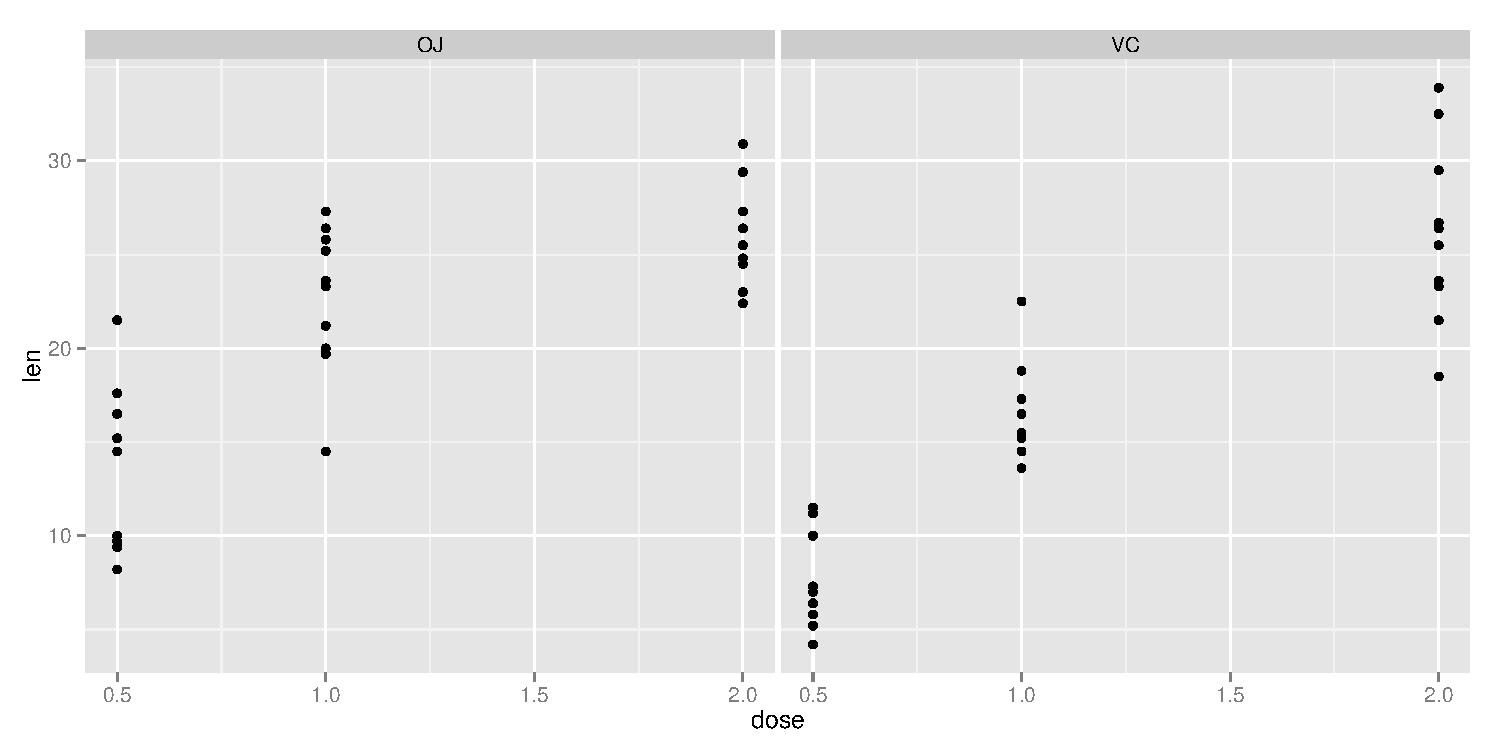
\includegraphics{BMT_project2_for_submission_20-04-2015_files/figure-latex/Quick simple plot-1.pdf}

Plot 2

\begin{Shaded}
\begin{Highlighting}[]
\NormalTok{## Plotting using boxplot}
\NormalTok{## function to label the plot facets for readability.}
\NormalTok{facet_names <-}\StringTok{ }\KeywordTok{list}\NormalTok{(}\StringTok{'OJ'}\NormalTok{=}\StringTok{"Orange Juice"}\NormalTok{, }\StringTok{'VC'}\NormalTok{=}\StringTok{"Ascorbic Acid"}\NormalTok{)}
\NormalTok{facet_labeller <-}\StringTok{ }\NormalTok{function(variable,value)\{ }\KeywordTok{return}\NormalTok{(facet_names[value]) \}}
\NormalTok{## NB : factor of dose required because ggplot requires factor (dose is numeric)}
\NormalTok{g <-}\StringTok{ }\KeywordTok{ggplot}\NormalTok{(ToothGrowth, }\KeywordTok{aes}\NormalTok{(}\KeywordTok{factor}\NormalTok{(dose), len, }\DataTypeTok{fill =} \KeywordTok{factor}\NormalTok{(dose))) +}
\KeywordTok{scale_fill_discrete}\NormalTok{(}\DataTypeTok{name=}\StringTok{"Dosage (mg)"}\NormalTok{) +}\StringTok{ }
\KeywordTok{geom_boxplot}\NormalTok{(}\DataTypeTok{outlier.colour =} \StringTok{"red"}\NormalTok{,}\DataTypeTok{outlier.shape =} \DecValTok{23}\NormalTok{, }\DataTypeTok{outlier.size =} \DecValTok{5}\NormalTok{) +}
\KeywordTok{geom_jitter}\NormalTok{(}\DataTypeTok{position=}\KeywordTok{position_jitter}\NormalTok{(}\DataTypeTok{w=}\FloatTok{0.2}\NormalTok{)) +}
\KeywordTok{facet_grid}\NormalTok{(.~supp, }\DataTypeTok{labeller=}\NormalTok{facet_labeller) +}
\KeywordTok{ylab}\NormalTok{(}\StringTok{"Tooth Growth"}\NormalTok{) +}
\KeywordTok{xlab}\NormalTok{(}\StringTok{"Dose (mg)"}\NormalTok{)+}
\KeywordTok{ggtitle}\NormalTok{(}\StringTok{"Tooth Growth vs Supplement Doses"}\NormalTok{)}
\NormalTok{## fill = factor(dose) : fills in boxplot with colour coding, easy to read graph}
\NormalTok{## geom_jitter - jitters points so we can see overlapping points. w=0.2 sets width of jitter.}
\NormalTok{## outlier - set properties so we can see points outside the values shown by the boxplot }
\NormalTok{## facet_grid - plot separate panels for each value of supp. ("OJ" &" "VC")}
\NormalTok{## scale_fill_discrete : sets legend title.}
\NormalTok{g  }
\end{Highlighting}
\end{Shaded}

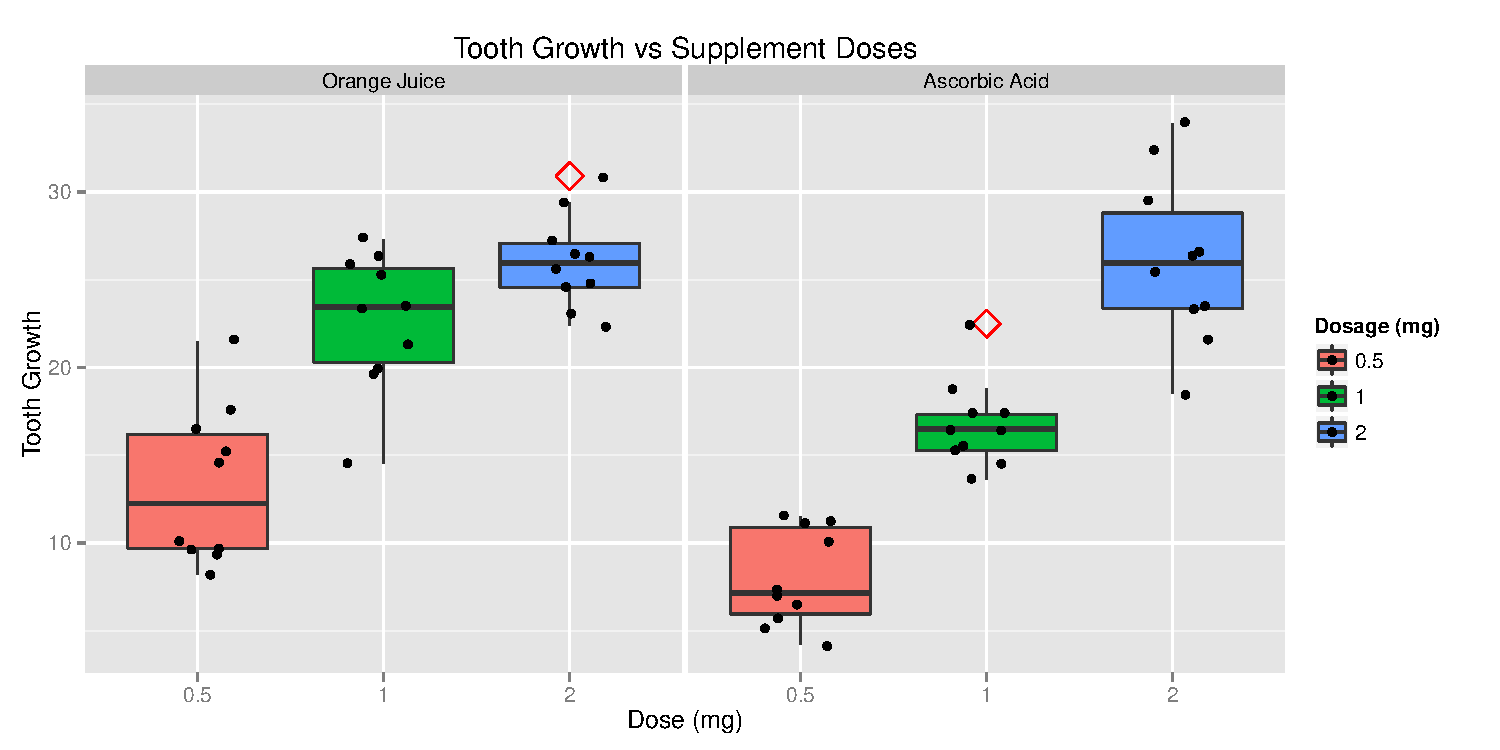
\includegraphics{BMT_project2_for_submission_20-04-2015_files/figure-latex/Plot for analysis-1.pdf}

\subsubsection{Assumptions}\label{assumptions}

The Analysis are based on the following assumptions.\\* The variances of
each test group are different. (ie: var.equal = FALSE)\\* The test
subjects are not related, ie: each test subject was tested with either
Orange Juice or Ascorbic Acid.\\* The test subjects were randomly
selected. There are no properties of the test subjects causing bias in
results.\\* The test subjects are independent and identically
distributed.\\\url{https://stat.ethz.ch/R-manual/R-devel/library/datasets/html/ToothGrowth.html}

Description : The response is the length of odontoblasts (teeth) in each
of 10 guinea pigs at each of three dose levels of Ascorbic Acid (0.5, 1,
and 2 mg) with each of two delivery methods (orange juice or ascorbic
acid).

Git url :
\url{https://github.com/aspiringguru/Statistical-Inference-Project.git}

\end{document}
